\documentclass{beamer}

\usepackage{listings}
\usetheme{Ilmenau}
%\usecolortheme{albatross}

\begin{document}

\title{Using Beamer for Presentations}
\subtitle{Tips and Tricks for Tech People}
\author{Joey Bernard}
\titlegraphic{
\includegraphics[width=\textwidth,height=.4\textheight]{dark.png}}

\begin{frame}
   \titlepage
\end{frame}

\usebackgroundtemplate{
\includegraphics[width=\paperwidth]{pool-water-texture.jpg}}

\begin{frame}
   \frametitle{My First Slide}
   \begin{itemize}
      \item point 1
      \item point 2
   \end{itemize}
\end{frame}

\begin{frame}
   \frametitle{Feeding Hummingbirds}
     \begin{columns}[t] % contents are top vertically aligned
     \begin{column}[T]{5cm} % each column can also be its own environment
   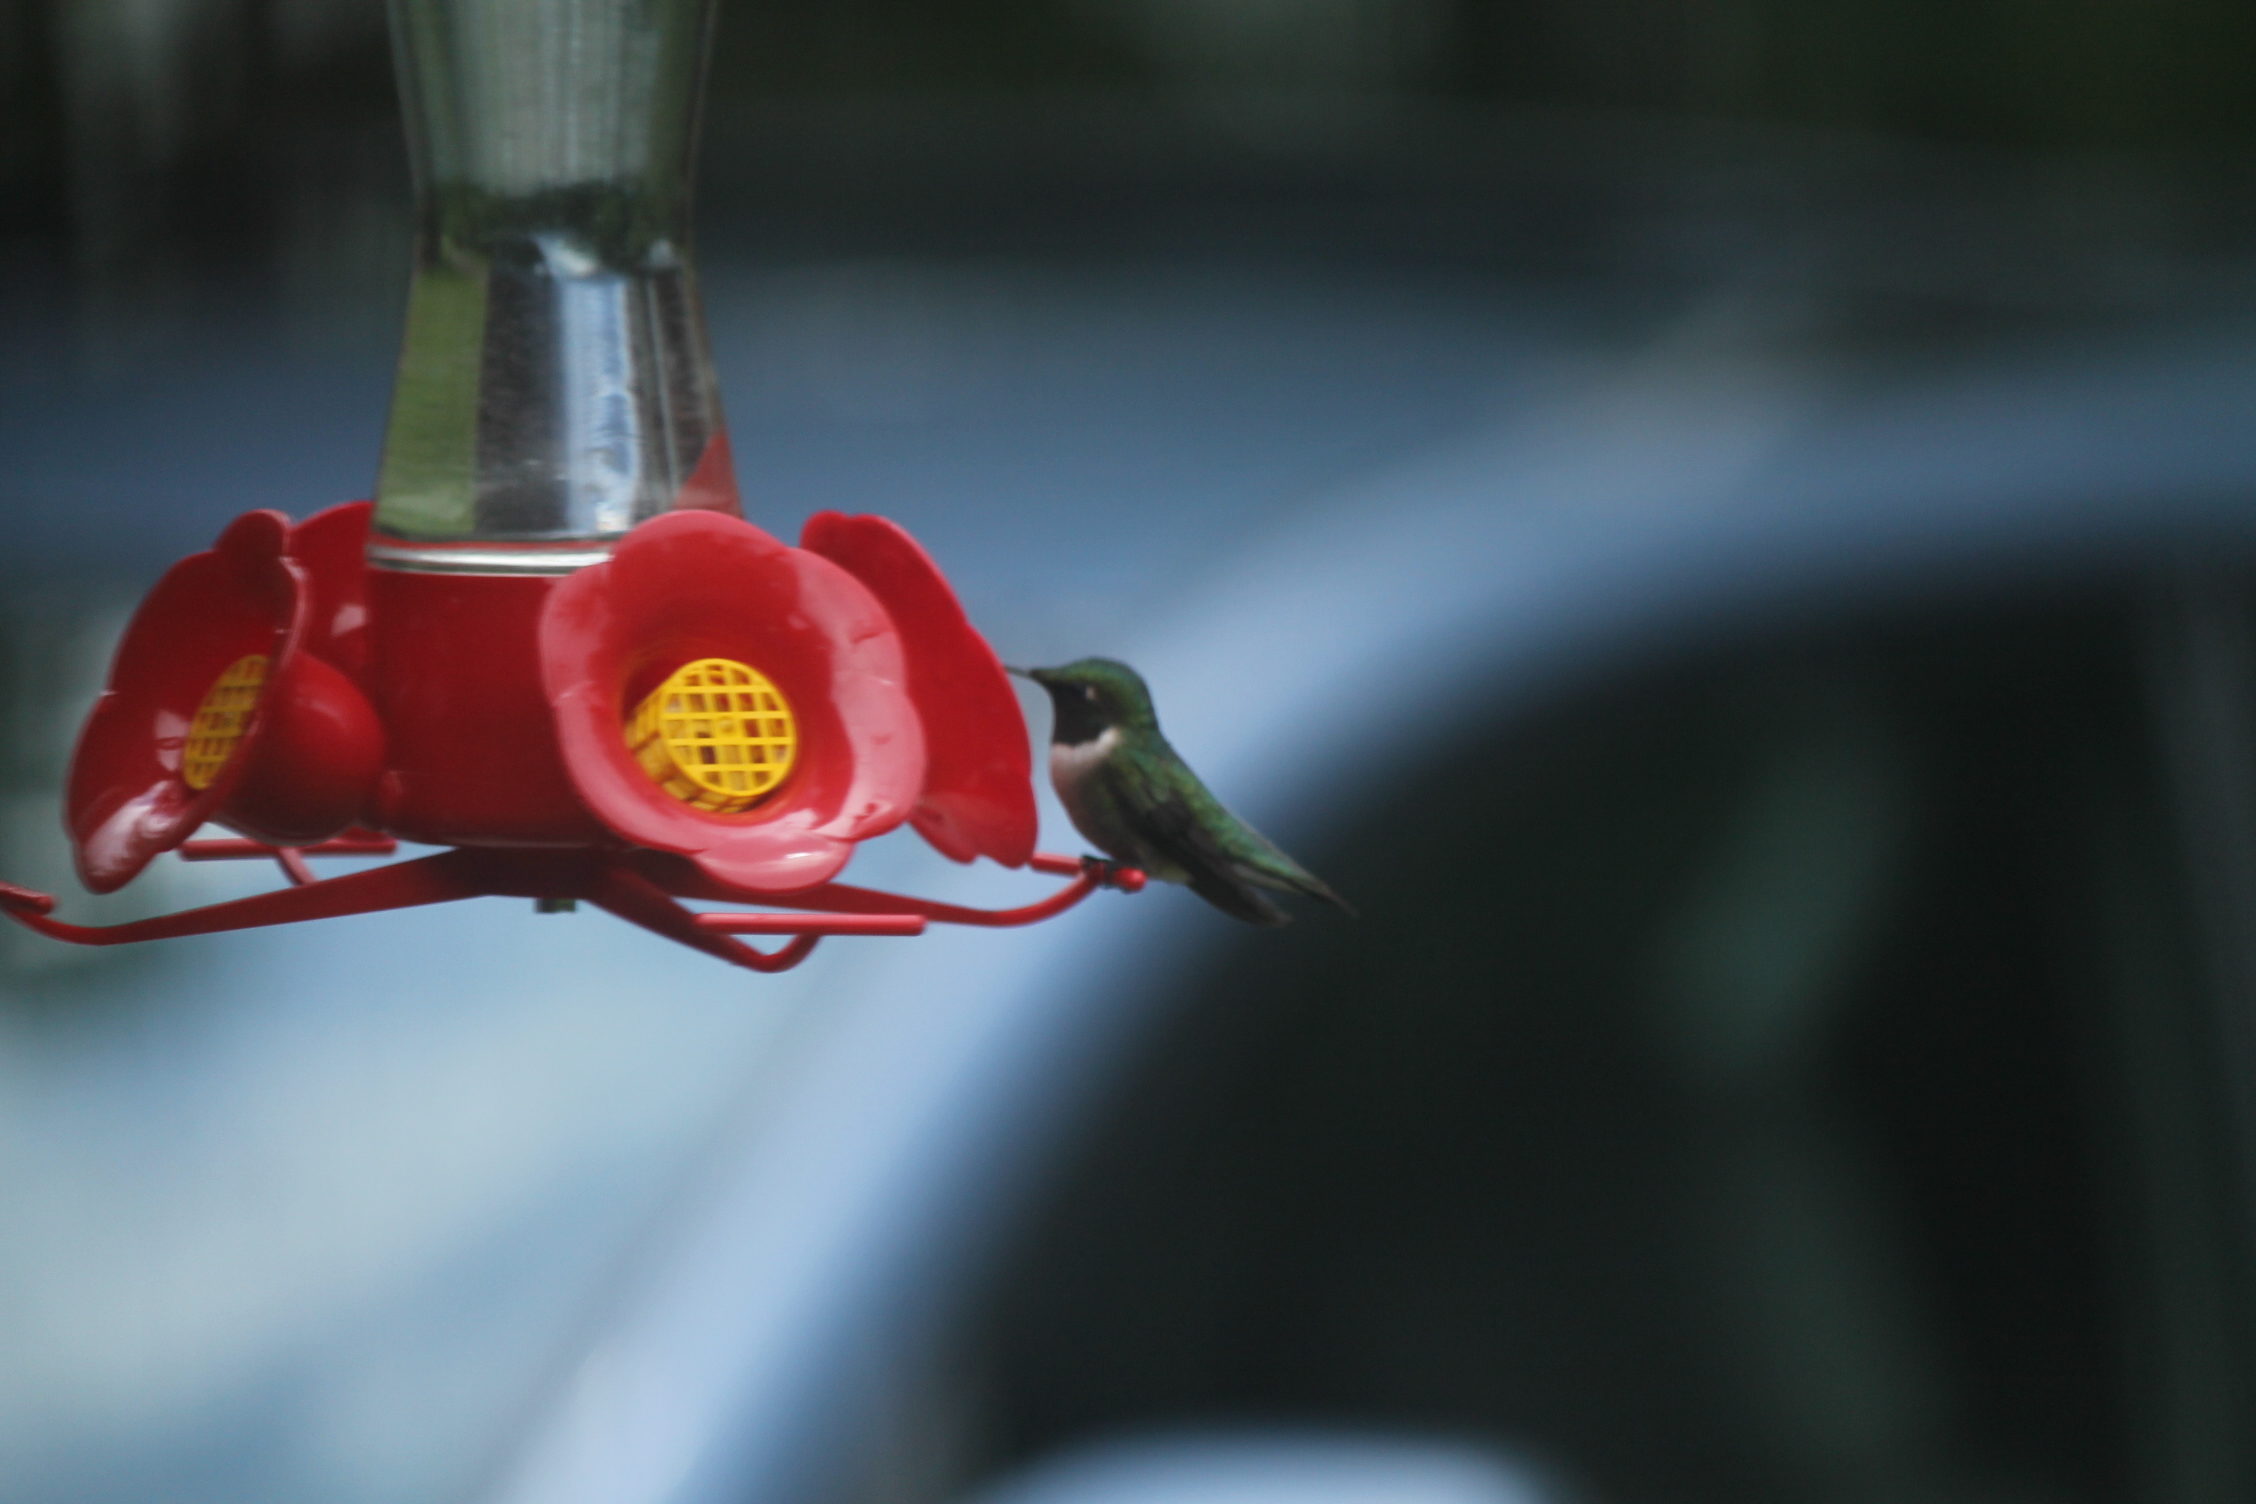
\includegraphics[width=\textwidth]{img_7991.jpg}
     \end{column}
     \begin{column}[T]{5cm} % alternative top-align that's better for graphics
        Feeding hummingbirds \\ is one way to help nature
     \end{column}
     \end{columns}

\end{frame}

\begin{frame}
   \frametitle{One Point at a Time}
   \begin{itemize}
      \item First one point
      \pause \item then another
      \pause \item and another
   \end{itemize}
\end{frame}

\begin{frame}
   \frametitle{More Control}
   \begin{itemize}
      \item<1-> This is displayed from slide 1 on
      \item<2> This is displayed only on slide 2
      \item<3-> This is displayed from slide 3 on
   \end{itemize}
\end{frame}

\begin{frame}[fragile]
   \frametitle{My Source Code}
   \begin{lstlisting}
int main() {
   printf(''This is my code\n'');
}
   \end{lstlisting}
\end{frame}

\end{document}
